% Created 2021-07-20 Tue 14:04
% Intended LaTeX compiler: pdflatex
\documentclass[presentation, xetex]{beamer}
\usepackage[utf8]{inputenc}
\usepackage[T1]{fontenc}
\usepackage{graphicx}
\usepackage{grffile}
\usepackage{longtable}
\usepackage{wrapfig}
\usepackage{rotating}
\usepackage[normalem]{ulem}
\usepackage{amsmath}
\usepackage{textcomp}
\usepackage{amssymb}
\usepackage{capt-of}
\usepackage{hyperref}
\usepackage{style}
\usetheme{default}
\author{佐野 仁}
\date{\today{}}
\title{Regular Model Cheching の紹介}
\subtitle{Parameteterized model verification}
\hypersetup{
 pdfauthor={佐野 仁},
 pdftitle={Regular Model Cheching の紹介},
 pdfkeywords={},
 pdfsubject={},
 pdfcreator={Emacs 27.2 (Org mode 9.4.4)}, 
 pdflang={English}}
\begin{document}

\maketitle



\section{Introduction}
\label{sec:orgdf394bb}

\begin{frame}[label={sec:org4775004}]{参考文献}
Handbook of Model Checking
\begin{itemize}
\item \url{https://link.springer.com/book/10.1007/978-3-319-10575-8}
\end{itemize}


この本の Chapter 21: Model Checing Parameteterized Systems を紹介する
\begin{itemize}
\item その中でも Section 3: Regular Model Checking を中心に扱う
\end{itemize}
\end{frame}


\begin{frame}[label={sec:orged5e662}]{背景:LMNtal のモデル検査}
SLIM は Model Checking が可能
\begin{itemize}
\item ただし,全状態を列挙しないと健全な検査はできない
\begin{itemize}
\item 無限の状態空間を持つモデル・パラメータの入ったモデルは\\
扱えない
\end{itemize}
\item 何らかの \alert{\alert{Abstraction}} を入れたい
\end{itemize}


LMNtal ShapeType は文脈自由の生成規則によって\\
生成されるモデルを検査可能
\begin{itemize}
\item 抽象化の仕組みを備えている
\item が,まだ未知数なものも多い(性能・表現力)
\end{itemize}
\end{frame}


\begin{frame}[label={sec:org15380e5}]{(とりあえずの)方針}
既存の \alert{\alert{Parameteterized Model Checking}} について調査し,\\
SLIM, LMNtal ShapeType などに応用できないか考える
\begin{itemize}
\item 今は調査の段階
\end{itemize}
\end{frame}


\section{Parametrized Model Checking の概要}
\label{sec:org7257787}

\begin{frame}[label={sec:org85469bf}]{Parametrized Model Checking とは}
パラメータの入ったモデルを扱う
\begin{itemize}
\item N 個のプロセスが相互排他制御を行うなど
\end{itemize}


パラメータに許される全ての値について,\\
モデルが仕様を満たすことを検証する
\begin{itemize}
\item 1 個のプロセスなら OK,2 個でも OK,3 個でも OK, \ldots{}
\item 無限のパターンが存在する場合もある
\end{itemize}
\end{frame}


\begin{frame}[label={sec:org72b5105}]{Parametrized Moel Checking の応用分野:}
\begin{itemize}
\item mutex のアルゴリズム
\item (CPU の) bus の protocol
\item Network protocol
\item Cache coherence protocol
\item web services
\item sensor network
\end{itemize}
\end{frame}


\begin{frame}[label={sec:org578ffe5}]{Parametrized Model Checking の重要なファクタ}
\begin{description}
\item[{Components}] プロセスは有限でないかも知れない
\item[{Topology}] システムはバラバラかも知れないし,直線状・リング・木・グラフかも知れない
\item[{Communication primitives}] \mbox{}\\
randezvous (二つ以上のものが同時に書き換わる)か\\
shared variable の書き換えか
\begin{itemize}
\item また,量化子 \alert{\alert{global condition}} が付くかも知れない
\end{itemize}
\end{description}
\end{frame}



\begin{frame}[label={sec:orgf82b670},fragile]{Parametrized Model Checking の簡単な例題}
 \begin{center}
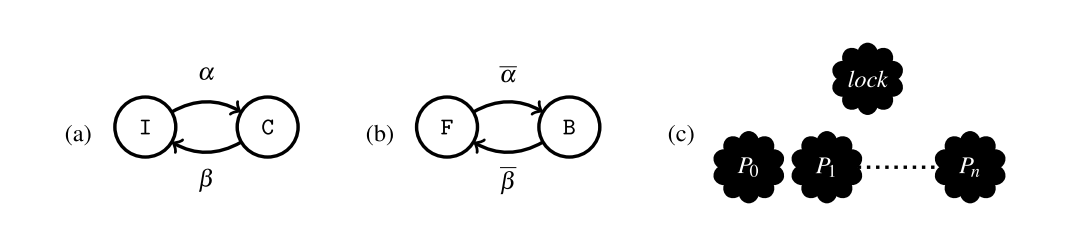
\includegraphics[width=.9\linewidth]{./images/simple-mutex.png}
\end{center}

\begin{itemize}
\item (a). 一つのプロセスの状態遷移
\begin{itemize}
\item \texttt{Initial state} \(\longleftrightarrow\) \texttt{Critical section}
\end{itemize}
\item (b). Lock の状態遷移
\begin{itemize}
\item \texttt{Free} \(\longleftrightarrow\) \texttt{Busy}
\end{itemize}
\item (c). Lock と n 個のプロセス
\end{itemize}
\end{frame}



\begin{frame}[label={sec:org990901c}]{PMC/Backward reachability}
これはBackward reachability で検証可能な例題
\begin{itemize}
\item 去年恒川さんが紹介したもの
\begin{itemize}
\item \url{https://www.ueda.info.waseda.ac.jp/localpage/seminars/wiki/index.php?plugin=attach\&refer=Schedule\%2F2020Autumn\&openfile=tsunekawa20201215.pdf}
\end{itemize}
\end{itemize}
\end{frame}



\begin{frame}[label={sec:orgf88bed0},fragile]{PMC and LMNtal ShapeType}
 ShapeType でも検証可能なはず
\begin{itemize}
\item 日誌に書いて,山本さんには話した
\item (でもダメだったらしい.調査が必要かも)
\end{itemize}


\begin{verbatim}
defshape ps {
  ps :- ps, i.
  ps :- lock.  % まだ誰もロックを獲得していない
  ps :- c.     % クリティカルセクションへ入った
}
acquire @@ i, lock :- c.
release @@ c :- i, lock.
\end{verbatim}
\end{frame}


\begin{frame}[label={sec:org2c533da}]{今回紹介するもの}
ただし,今回はこれよりももっと難しい例題を扱える,\\
Regular Model Checking を紹介する
\begin{itemize}
\item 直線・リング状のシステムを扱える
\item 遷移規則に量化子をつけることもできる
\end{itemize}
\end{frame}


\section{Regular Model Checking の導入}
\label{sec:org0d3c127}

\begin{frame}[label={sec:org6d41556}]{Regular Model Checking の概要}
リングや直線状の形状をしており,\\
隣接したプロセス間で通信しあうシステムを検証できる
\begin{itemize}
\item 今回扱うのは直線状のもの
\end{itemize}



直線状のシステムでは,その位置を優先度と見做して検査可能
\begin{itemize}
\item 優先度付きのプロトコルの検証が可能
\end{itemize}


\hspace{1em}

RMC において \alert{\alert{safety property は決定可能ではない}}
\begin{itemize}
\item Acceleration technique などを用いることで\\
解けるようになる問題はある
\end{itemize}
\end{frame}


\begin{frame}[label={sec:org9bb2889}]{Regular Model Checking の非形式的な定義}
\begin{description}
\item[{それぞれのプロセスの local な state}] finite alphabet で表す
\begin{itemize}
\item e.g. \(\{a, b, c\}\)
\end{itemize}
\item[{システムの構成}] word(文字列)で表す
\begin{itemize}
\item e.g. \(abbc\) : 一番目のプロセスは状態 \(a\),二番目のプロセスは状態 \(b\),\ldots{}
\end{itemize}
\item[{システムの構成の集合}] finite automata(または正規表現) で表す
\begin{itemize}
\item e.g. \(ab^*c\)
\end{itemize}
\item[{遷移 = \alert{\alert{finite-state transducer}}}] \mbox{}\\
ある状態からある状態へ遷移するか判定する\\
finite automata
\begin{itemize}
\item e.g. \(abbc\) は \(abcc\) に遷移可能か? \thusmark yes/no
\end{itemize}
\end{description}
\end{frame}


\begin{frame}[label={sec:org4e6893d}]{関係 \(R\) に関する形式的な定義}
\begin{itemize}
\item \(\Sigma\) は \alert{\alert{alphabet}} の有限集合.
\item 関係 \(R \subseteq \Sigma \times \Sigma\) と集合 \(A \subseteq \Sigma\) に対して,\\
\(A \circ R := \{b | \exists a. (a \in A) \land ((a, b) \in R)\}\) を定義する
\begin{itemize}
\item 要は \(A\) に含まれている状態から遷移できる状態の集合
\end{itemize}
\item 関係 \(R, R' \subseteq \Sigma \times \Sigma\) に対して,合成
\(R \circ R' := \{(a_1, a_2) | \exists b. ((a_1, b) \in R) \land ((b, a_2) \in R')\}\)
を定義する
\item \(R^0 = \{(a, a) | a \in \Sigma\}\), \(R^{i + 1} = R^i \circ R\) と定義する
\item \(R^* := \bigcup_{i \geq 0} R^i\), \(R^+ := \bigcup_{i \geq 1} R^i\)
\end{itemize}
\end{frame}


\begin{frame}[label={sec:org18574a2}]{Transducer \(T\) の形式的な定義}
\(\Sigma\) 上の transducer \(T\) は \\
\((Q, q_{init}, \Delta, F)\) なる四つ組の有限状態オートマトン
\begin{description}
\item[{有限状態}] \(Q\)
\item[{初期状態}] \(q_{init} \in Q\)
\item[{遷移関係}] \(\Delta \subseteq Q \times (\Sigma \times \Sigma) \times Q\)
\begin{itemize}
\item \((\Sigma \times \Sigma)\) なのは,入力に alphabet を二つ受け取って,状態遷移するから
\end{itemize}
\item[{受理状態}] \(F \subseteq Q\)
\end{description}
\end{frame}



\begin{frame}[label={sec:org5ba6bcd},fragile]{例題:トークンパッシング}
 \begin{center}
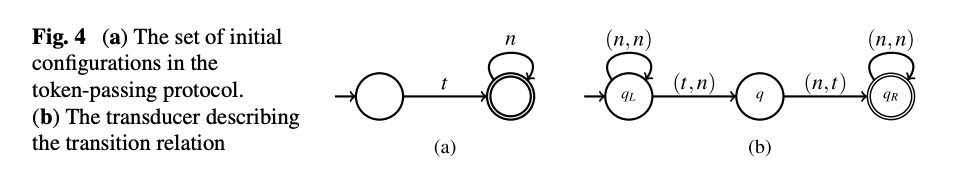
\includegraphics[width=.9\linewidth]{./images/token-example.png}
\end{center}


トークン \texttt{t} を左から右に垂れ流すだけの例題
\begin{itemize}
\item 初期状態では一番左のみ \texttt{t} が存在する
\item \texttt{t} を一つ右にずらす遷移を認める transducer も定義
\end{itemize}
\end{frame}



\begin{frame}[label={sec:org91d7a9f},fragile]{Transducer \(T\) が受理するもの}
 Transducer は \((\Sigma \times \Sigma)\) 上の有限長の列 \\
\((a_1, b_1)(a_2, b_2) \dots (a_n, b_n)\) を受理する
\begin{itemize}
\item Transducer が受理するものを言語 \(L(T)\) と呼ぶ
\item また,Transducer が受理するものを \texttt{unzip} した二つの文字列は \\
Regular relation \(R(T)\) であると定義する
\begin{itemize}
\item \((a_1, b_1) \dots (a_n, b_n) \in L(T)\) なら,\((a_1 \dots a_n, b_1 \dots b_n) \in R(T)\)
\item システムの遷移関係を表す
\end{itemize}
\end{itemize}
\end{frame}



\begin{frame}[label={sec:orgd4e213e}]{例題:トークンパッシングにおける transducer}
\begin{center}
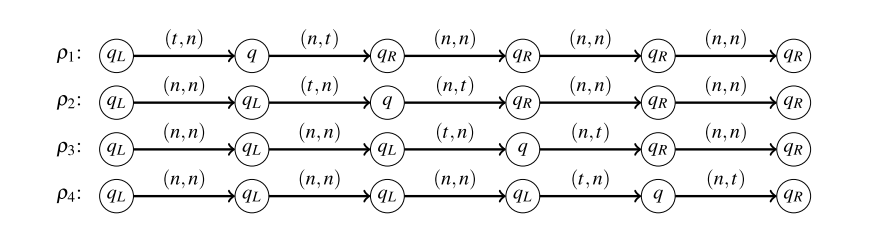
\includegraphics[width=0.7\textwidth]{./images/four-transducer.png}
\end{center}


\begin{description}
\item[{\(\rho_1, \dots, \rho_4\)}] Transducer にそれぞれ異なる入力を与えて\\
走らせた結果
\item[{わかること}] システムには \dots{}
\begin{enumerate}
\item \((t, n)(n, t)(n, n)(n, n)(n, n)\) という遷移が許される
\begin{itemize}
\item \((tnnnn, ntnnn) \in R(T)\)
\end{itemize}
\item \((n, n)(t, n)(n, t)(n, n)(n, n)\) という遷移も OK
\begin{itemize}
\item \((ntnnn, nntnn) \in R(T)\) は OK
\end{itemize}
\item \dots{}
\end{enumerate}
\end{description}
\end{frame}


\begin{frame}[label={sec:org25b9cdf}]{Regular relation \(R(T)\) に関する略記法}
\begin{itemize}
\item \((R(T))^+\) の代わりに,\(R^+(T)\) と書くことにする
\item 同様に,\(R^+(T), R^*(T), R^i(T)\) と書く
\end{itemize}
\end{frame}


\begin{frame}[label={sec:org4e3539e}]{例題:トークンパッシングの \(R(T)\) の推移}
\begin{center}
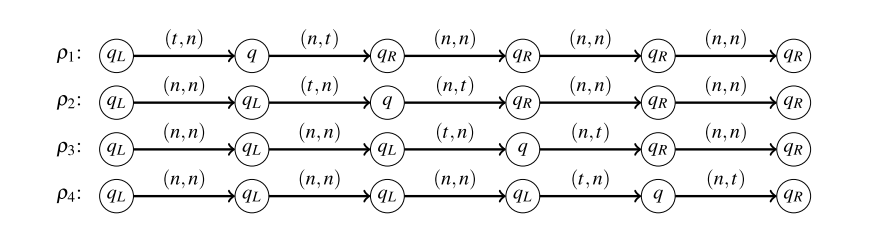
\includegraphics[width=0.7\textwidth]{./images/four-transducer.png}
\end{center}

\((tnnnn, ntnnn), (ntnnn, nntnn), \dots, (nnntn, nnnnt) \in R(T)\)
\begin{itemize}
\item 従って, \((tnnnn, nnnnt) \in R^4(T)\)
\end{itemize}
\end{frame}




\section{Acceleration Techniques の導入}
\label{sec:orgcae6314}

\begin{frame}[label={sec:orgb06f3d3}]{RMC でそもそも何をしたいのか}
RMC の一般的な課題は,\\
Transducer relation から推移閉包を求めること
\begin{itemize}
\item transducer \(T\) から,\(R(T^+) = R^+(T)\) となる \(T^+\) を求めたい
\item 要は到達可能な全ての状態への遷移を受理する \\
transducer が知りたい

\(T^+\) さえ求まれば,到達可能な状態に \\
仕様を満たさないものが存在しないか(safe)が判定できる
\begin{itemize}
\item 次ページから
\end{itemize}
\end{itemize}
\end{frame}


\begin{frame}[label={sec:org1163416}]{RMC での Safety の検証}
入力
\begin{description}
\item[{初期状態}] regular set of initial configuration \(I\)
\item[{違反状態}] regular set of bad configuration \(B\)
\item[{遷移規則}] transducer \(T\)
\end{description}

を与えられて,
\begin{itemize}
\item \(I\) から \(R(T)\) を辿って,
\(B\) へ到達できるパスが存在するか?
\end{itemize}
を計算する
\end{frame}


\begin{frame}[label={sec:org8b1a01e}]{例題:トークンパッシング}
\begin{center}
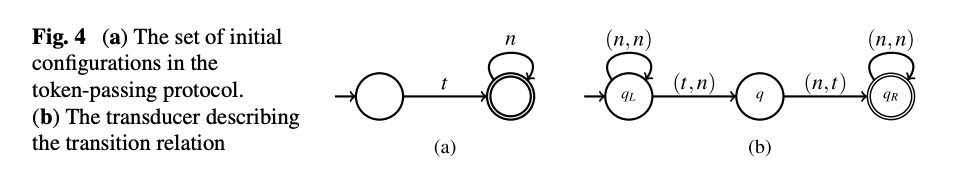
\includegraphics[width=.9\linewidth]{./images/token-example.png}
\end{center}


regular set of initial configuration \(I\) は
\begin{itemize}
\item \(t n^*\)
\end{itemize}


regular set of bad configuration \(B\) は
\begin{itemize}
\item \((t + n)^* t (t + n)^* t (t + n)\)
\item トークンが二つ以上ある状態はエラー
\end{itemize}
\end{frame}



\begin{frame}[label={sec:org13a4ba7}]{RMC のフレームワークについてもう少し詳しく}
RMC は
\begin{enumerate}
\item \(Inv = I \circ R^*(T)\) を計算して
\item \(Inv \cup B = \emptyset\) であるかを確認する
\end{enumerate}


\(R^*(T) = \{(a, a) | a \in \Sigma\} \cup R(T^+)\) なので
\alert{\alert{\(T^+\) さえ計算できれば良い}}


Transducer \(T\) が与えられた時に,\(R^+(T)\) は一般に計算不可能
\begin{itemize}
\item そもそも有限でない可能性もある
\item なので,(\(R^+(T)\) ではなく)\(T^+\) を計算する手法,\\
\alert{\alert{Acceleration}} を紹介する
\end{itemize}
\end{frame}


\begin{frame}[label={sec:orgad46fa7}]{例題: transducer の推移}
\begin{center}
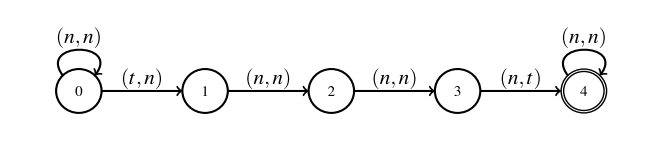
\includegraphics[width=.9\linewidth]{./images/3-transducer.png}
\end{center}

例題において,\(T^n\) は n 回トークンが右に伝わるような遷移

transducer \(T^3\) は上図のようになる
\begin{itemize}
\item トークンを三つ右にずらす遷移(を受理する)
\item \((n^* \; tnn \; n^*, n^* \; nnt \; n^*) = R^3(T) = R(T^3)\)
\end{itemize}
\end{frame}



\begin{frame}[label={sec:org360dbf4}]{例題における推移閉包}
\begin{center}
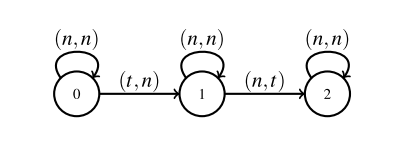
\includegraphics[width=.9\linewidth]{./images/n-transitive-transducer.png}
\end{center}

\(T^+\) はトークンが一回以上右に伝わるような全ての遷移(を受理する)
\begin{itemize}
\item \((n^* \; t \; n^* \; n^* , n^* \; n^* \; t \; n^*) = R^+(T) = R(T^+)\)
\end{itemize}
\end{frame}



\begin{frame}[label={sec:orge948584}]{推移の計算}
もちろん \(T^n\) を \(n = 1, 2, 3, \dots\) について \\
全て計算するわけにはいかない
\begin{itemize}
\item \(R^+(T)\) を受理する \emph{column transducer} \(T^{col}\) を導入する
\end{itemize}
\end{frame}


\begin{frame}[label={sec:orge6f662f}]{Column Transducer}
Transducer \(T\) を与えられた時に,
\begin{description}
\item[{Column transducer}] \mbox{}\\
\(T^{col}\) は \(R^+(T)\) を受理する transducer
\item[{Quotienting}] \mbox{} \\
同値関係 \(\simeq\) を定めて, \\
同値類は代表元にまとめる(圧縮する)ことで効率化
\end{description}
\end{frame}


\begin{frame}[label={sec:orgc03602b}]{Column Transducer の例}
\begin{center}
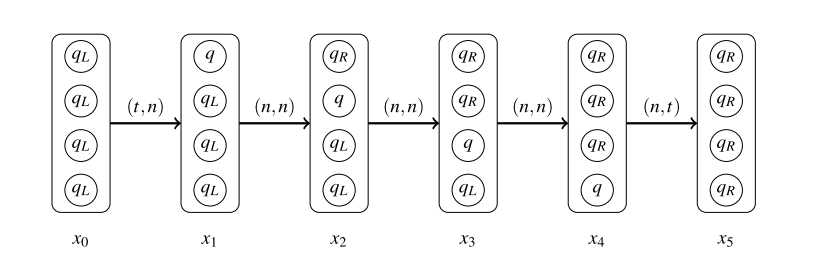
\includegraphics[width=0.6\textwidth]{./images/column-transducer.png}
\end{center}

\begin{itemize}
\item これを一回走らせるだけで, \\
\(\rho_1, \rho_2, \rho_3, \rho_4\) をこの順番に実行した結果をシミュレートできる
\end{itemize}


\(T^{col}\) の状態は \(Q\) の要素の列であり column と呼ぶ
\begin{itemize}
\item 図の角丸の枠で囲んであるもの
\item column が高さ i のとき,\(T^{col}\) は \\
\(R^i(T)\) が受理する文字列のペアを \alert{\alert{一回実行するだけで}} 受理する
\end{itemize}
\end{frame}




\begin{frame}[label={sec:org78ba19a}]{Column Transducer の形式的定義}
Transducer \(T\) が与えられたとき,
column transducer は  \(T^{col} = (Q^{col}, q_{init}^{col}, \Delta^{col}, F^{col})\) の四つ組
\begin{description}
\item[{\(Q^{col} = Q^+\)}] \(T\) の状態の空でない列の集合
\item[{\(q_{init}^{col} = q_{init}^+ \subseteq Q^{col}\)}] \(T\) の初期状態の空でない列の集合
\item[{\(\Delta^{col} \subseteq Q^{col} \times (\Sigma \times \Sigma) \times Q^{col}\)}] は以下のように定義される
\begin{itemize}
\item for any columns \(x_1 = q_1 q_2 \dots q_m\) and \(x_2 = r_1 r_2 \dots r_m\) and a pair (\(a, a')\),
\item we have \((x_1, (a, a'), x_2) \in \Delta^{col}\)
\item if there exist \(a_0, a_1, \dots, a_m\) with \(a = a_0\) and \(a' = a_m\)
\item such that \(q_i \overset{(a_{i - 1}, a_i)}{\longrightarrow_T} r_i\)
\item for \(1 \leq i \leq m\)
\end{itemize}
\end{description}
\end{frame}


\section{Quotienting}
\label{sec:org3587ef3}

\begin{frame}[label={sec:orgeeab133}]{Quotieting のモチベーション}
Column transducer の問題は \alert{\alert{無限の状態数を持つ}} 可能性があること
\begin{itemize}
\item Explicit に生成することはできない
\item \(T^{col}\) の column \(Q^{col}\) の集合を,\\
合同関係 \(\simeq\) を用いて \alert{\alert{商集合}} で扱えば良さそう
\begin{itemize}
\item これを \alert{\alert{Quotienting}} と呼ぶ
\end{itemize}
\end{itemize}
\end{frame}



\begin{frame}[label={sec:org2c0415e}]{Left/right-copying}
状態 \(q \in Q\) は以下のような場合に \alert{\alert{left-copying}} という

全ての次のような遷移
\begin{itemize}
\item \(q_{init} \overset{(a_0, a'_0)}{\longrightarrow_T} q_1 \overset{(a_1, a'_1)}{\longrightarrow_T} \dots \overset{(a_{n-1}, a'_{n-1})}{\longrightarrow_T} q_n\)
\item ただし \(q_n = q\)
について,
\begin{itemize}
\item \(a_i = a'_i\) for all \(i \in \{0, 1, \dots, n - 1\}\)
\end{itemize}
\end{itemize}


\hspace{1em}


right-copying も同様に定義する
\end{frame}

\begin{frame}[label={sec:orgbd617d3}]{left/right-copying な状態の表現}
要するに,left-copying の状態の prefix はただ入力を出力へコピーして流すだけ

\begin{itemize}
\item left-copying な状態を \(q_L\),
\item right-copying な状態を \(q_R\),
\item left/right-copying な状態の集合を \(Q^{copy}\)
と表す
\end{itemize}
\end{frame}


\begin{frame}[label={sec:org35ea663}]{合同関係 \(\simeq\) の定義}
こうした \alert{\alert{ただコピーするだけのもの}} を無視して\\
等価性を判定するというのが今回採用する同値関係
\begin{itemize}
\item 例えば,
\(q_L q_L x q_R\)
は
\(q_L x q_R q_R\)
と合同である
\end{itemize}
\end{frame}



\begin{frame}[label={sec:org84a8a12}]{\(\simeq\) 上の同値類の形式的定義}
\(\simeq\) 上の同値類は \(e_1 e_2 \dots e_n\) の形をした \alert{\alert{正規表現}} で表す
\begin{itemize}
\item ただし,\(e_i\) は以下の3つのうちのどれかの形になる

\begin{enumerate}
\item \(q_L^+\), for some left-copying state \(q_L\)

\item \(q_R^+\), for some left-copying state \(q_R\)

\item \(q\), for some state \(q\) which is neither left/right-copying
\end{enumerate}
\end{itemize}


\begin{itemize}
\item さらに,冗長な表現は許さない
\begin{itemize}
\item left/right copying かつ,\\
構文的に等しい正規表現 \(e_i\) が連続して現れるということはない
\end{itemize}
\end{itemize}


もちろん well-formed になっている
\begin{itemize}
\item 同じもの(同値類)は同じ表現(代表元)に落ちるはず
\end{itemize}
\end{frame}



\begin{frame}[label={sec:org15b2ec4}]{\(\simeq\) 上の同値類の形式的定義}
column \(x\) について,\([x]_\simeq\) で \(x\) の同値類を表す
\begin{itemize}
\item \(X, Y\), etc で column の同値類の集合(商集合)を表す
\end{itemize}
\end{frame}



\section{Quotient Transducer の導入}
\label{sec:org32cc1a9}

\begin{frame}[label={sec:org06b5ccb}]{Quotient Transducer の概要}
\(Q^{col}\) 上の同値関係 \(\simeq\) も定義できたので,\\
この同値関係を使って,また transducer を定義する
\begin{itemize}
\item 要するに, \alert{\alert{各々の状態が正規表現である automata}} を構築する
\end{itemize}
\end{frame}


\begin{frame}[label={sec:org2d5538e}]{Quotient Transducer の形式的定義}
\alert{\alert{Quotient transducer}} は \(T^\bullet = (Q^\bullet, q_{init}^\bullet, \Delta^\bullet, F^\bullet)\) の四つ組
\begin{description}
\item[{\(Q^\bullet \subseteq Q^{col}/_{\simeq}\)}] columns の同値類の集合
\item[{\(q_{init}^\bullet = q_{init}^+\)}] 初期状態の同値類の集合
\begin{itemize}
\item ただし,初期状態は left-copying だと仮定する
\end{itemize}
\item[{\(\Delta^\bullet \subseteq Q^\bullet \times (\Sigma \times \Sigma) \times Q^\bullet\)}] 以下のように定義される遷移
\begin{itemize}
\item For any columns \(x,x'\) and symbols \(a,a'\),
\item if \((x,(a,a'),x') \in \Delta\)
\item then \(([x]_\simeq, (a, a'), [x']_\simeq) \in \Delta^\bullet\).
\end{itemize}
\item[{\(F^\bullet = F^{col}/_\simeq\)}] 同値関係 \(\simeq\) で \(F^{col}\) を分割したもの
\end{description}
\end{frame}



\begin{frame}[label={sec:org6a99d21}]{Quotient Transducer の生成}
\(T^{col}\) ,つまり \(R^+(T)\),と同じものを受理する transducer を生成したい
\begin{itemize}
\item ただし,\(T^\bullet\) が \alert{\alert{finite state transducer かはわからない}}
\begin{itemize}
\item 無限に発散するかも
\end{itemize}
\item (仕方がないので) \(T^\bullet\) が \\
finite state であった場合には停止する手続きを考える
\begin{itemize}
\item つまり,この手法は \alert{\alert{完全ではない}} (アルゴリズムではない)
\end{itemize}
\end{itemize}
\end{frame}



\begin{frame}[label={sec:orgcc08749}]{前提とする定義:演算子}
\begin{enumerate}
\item 状態 \(q \in Q\) に対して \(q^\oplus\) を以下のように定義する
\begin{itemize}
\item \(q \in Q^{copy}\) なら \(q^\oplus := q^+\)
\item \(q \in Q^{copy}\) でないなら \(q^\oplus := q\)
\end{itemize}

\item 演算子 \(\star\) を以下のように同値類の結合と定義する
\begin{itemize}
\item \([x]_\simeq \star [y]_\simeq = [x \cdot y]_\simeq\)
\item ただし, \(\cdot\) は column を結合する演算子
\item より正確な定義は次ページ
\end{itemize}
\end{enumerate}


あとで例も出します
\end{frame}


\begin{frame}[label={sec:org02b46ea}]{\(\star\) の正確な定義}
2 に関してもっと正確には
\begin{itemize}
\item colum の同値類を正規表現 \(e_1 \dots e_n\), \(f_1 \dots f_m\) で表現したとき
\item \((e_1 \dots e_n) \star (f_1 \dots f_m)\) は
\begin{itemize}
\item \(e_n, f_1\) が両方とも left/right-copying な状態 \(q\) の \(q^+\)
と等しい場合は,
\(e_1 \dots e_n \cdot f_2 \dots f_m\)
\item そうではない場合は
\(e_1 \dots e_n \cdot f_1 \dots f_m\)
\end{itemize}
\end{itemize}


あとで例も出します
\end{frame}


\begin{frame}[label={sec:org1ec1f27}]{Quotient transducer の遷移規則}
同値類の集合 \(X, Y\) について,以下のどちらか満たすとき,
\(X \overset{(a, b)}{\longrightarrow_\bullet} Y\) と帰納的に定義する
\begin{enumerate}
\item \(x \overset{(a, a')}{\longrightarrow_T} y\),
\(X = x^\oplus\) かつ \(Y = y^\oplus\)
\item \(X = X_1 \star X_2\), \(Y = Y_1 \star Y_2\),
\(X \overset{(a, b)}{\longrightarrow_\bullet} X\) かつ
\(Y \overset{(b, a')}{\longrightarrow_\bullet} Y\)
\end{enumerate}


あとで例も出します
\end{frame}


\begin{frame}[label={sec:org282529c}]{例題:トークンパッシング}
\begin{center}
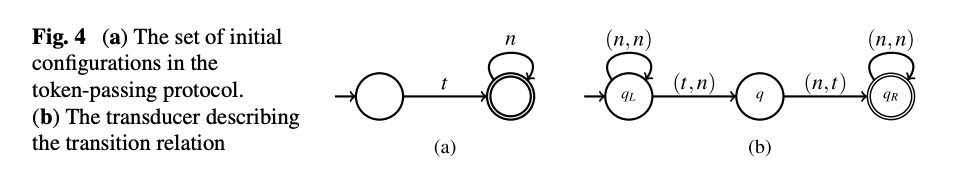
\includegraphics[width=.9\linewidth]{./images/token-example.png}
\end{center}

\begin{enumerate}
\item \(q_L^+ \overset{(t, n)}{\longrightarrow_T} q\) から
\(q_L^\oplus \overset{(t, n)}{\longrightarrow_T} q^\oplus\) なので
\(q_L^+ \overset{(t, n)}{\longrightarrow_\bullet} q\)

\item \(q_L^+ \overset{(n, n)}{\longrightarrow_T} q_L^+\) から
\(q^\oplus \overset{(n, n)}{\longrightarrow_T} q^\oplus\) なので
\(q_L^+ \overset{(n, n)}{\longrightarrow_\bullet} q_L^+\)
\end{enumerate}
\end{frame}



\begin{frame}[label={sec:orgdfabaae}]{例題:トークンパッシング}
\begin{center}
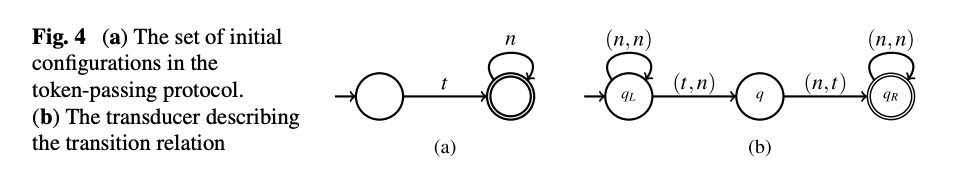
\includegraphics[width=.9\linewidth]{./images/token-example.png}
\end{center}


\begin{enumerate}
\setcounter{enumi}{2}
\item \(\underbrace{q_L^+ \overset{(t, n)}{\longrightarrow_\bullet} q}_{\hspace{0.3em}\circled{1}}\)  と
\(\underbrace{q_L^+ \overset{(n,n)}{\longrightarrow_\bullet} q_L^+}_{\hspace{0.3em}\circled{2}}\)
から \\
\(q_L^+ \star q_L^+ \overset{(t, n)}{\longrightarrow_\bullet} q \star q_L^+\)  なので \\
\(q_L^+ \overset{(t, n)}{\longrightarrow_\bullet} q q_L^+\)
\end{enumerate}
\end{frame}



\section{Quotient Transducer の生成手続き}
\label{sec:orga588c18}

\begin{frame}[label={sec:org1744cb6}]{Quotient Transducer の生成手続き}
\begin{center}
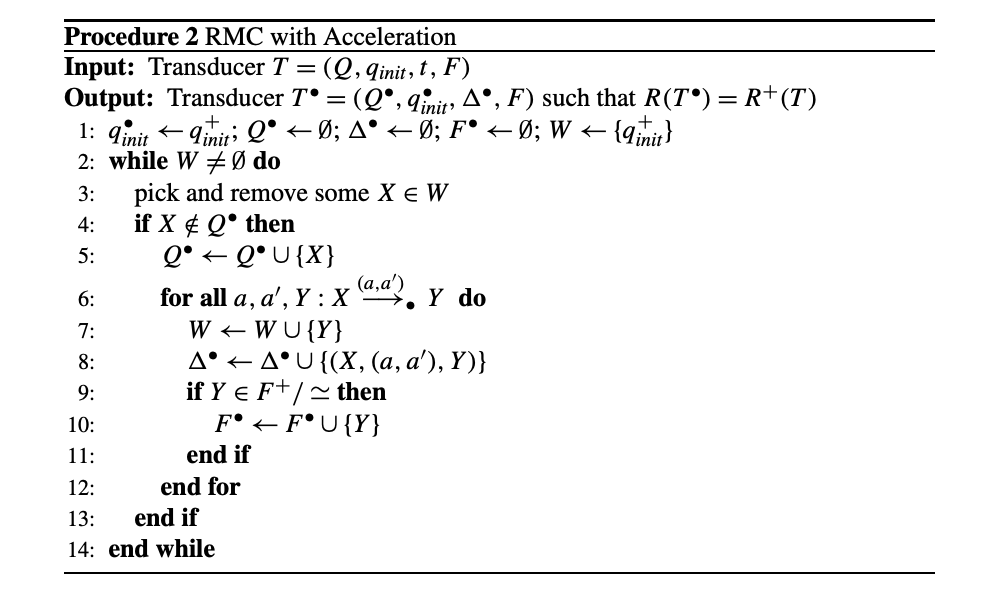
\includegraphics[width=0.7\textwidth]{./images/quoting-rmc.png}
\end{center}

\footnotesize
\begin{itemize}
\item W はまだ遷移先を計算していない状態の同値類(= 正規表現)の集合
\begin{itemize}
\item \footnotesize
W が空になったら計算終了
\item \footnotesize
W が空になるまで状態の同値類をポップして,\\
\(\longrightarrow_\bullet\) の先にあるものを追加していく
\end{itemize}
\end{itemize}
\end{frame}



\begin{frame}[label={sec:org16324ba}]{Quotient Transducer の生成手続きの適用例}
\begin{enumerate}
\item まずは初期状態 \(q_L^+\) を W に追加
\item W から \(q_L^+\) を選択.
\begin{enumerate}
\item \(q_L^+ \overset{(t,n)}{\longrightarrow_\bullet} q\) なので,
\(q\) を W に追加,
また, \((q_L^+, (t, n), q)\) を \(\Delta^\bullet\).
\item \(q_L^+ \overset{(t, n)}{\longrightarrow_\bullet} q\) と
\(q_L^+ \overset{(n,n)}{\longrightarrow_\bullet} q_L^+\)
から
\(q_L^+ \overset{(t, n)}{\longrightarrow_\bullet} q q_L^+\) なので\textsubscript{前に紹介した例題を参照}\\
\(q q_L^+\) を W に追加,
\((q_L^+ \overset{(t, n)}{\longrightarrow_\bullet} q q_L^+)\) を \(\Delta^\bullet\) に追加.
\end{enumerate}
\item W から \(q\) を選択.
\begin{enumerate}
\item \(q \overset{(n,t)}{\longrightarrow_\bullet} q_R^+\) なので
\(q_R^+\) を W に追加,
\((q, \overset{(n, t)}{\longrightarrow_\bullet}, q_R^+)\)
を \(\Delta^\bullet\) に追加.
\item \(q_R^+ \in F/_\simeq\) なので \(q_R^+\) を \(F^\bullet\) に追加
\end{enumerate}
\item \ldots{}
\end{enumerate}
\end{frame}


\begin{frame}[label={sec:orgf0d908c}]{Quotient Transducer の生成手続きの適用結果}
\begin{center}
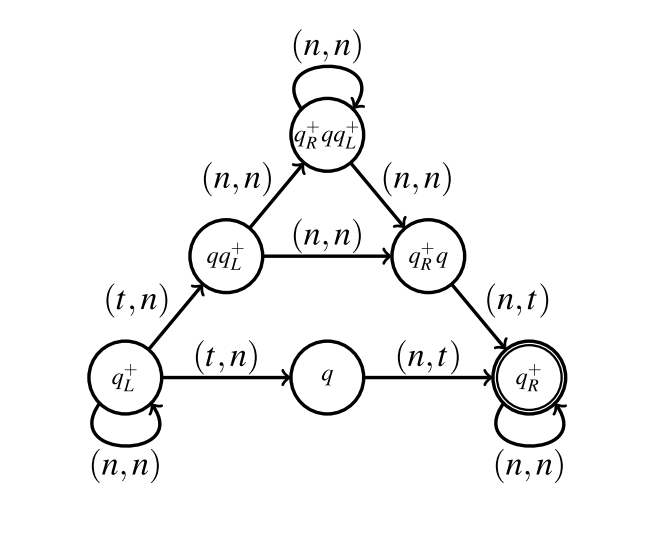
\includegraphics[width=0.5\textwidth]{./images/quoting-rmc-result.png}
\end{center}

\begin{itemize}
\item この transducer は \((n, n)^* (t, n) (n, n)^* (n, t) (n, n)^*\) を受理する
\item 正規表現の包含関係を計算するのは簡単にできるので,
safety の検証, \((I \odot R^*(T)) \cup B = \emptyset\) かどうかの確認,はすぐにできる
\end{itemize}
\end{frame}


\section{Monotomic Abstraction}
\label{sec:orgbf9d18d}

\begin{frame}[label={sec:orga879f40}]{Monotomic Abstraction とは}
推移閉包を正確に計算することが難しい場合は \\
\alert{\alert{over approximation}} を行う
\begin{itemize}
\item 次に紹介する例では,\\
wqo を適用できるように過大近似して検証している
\begin{itemize}
\item Backward reachability などが適用できる
\end{itemize}
\item もちろん false positive はありうる
\end{itemize}


今回は例題を見せるだけで手法は紹介しません
\end{frame}


\begin{frame}[label={sec:org5aff0f2}]{量化子付きの RMC}
全称量化付きの遷移規則を持つシステムの RMC を \\
直接行うのは難しい
\begin{itemize}
\item 全称量化子のことを(若干)無視して検証する
\item 余計に遷移してしまうかもしれないので完全ではない
\begin{itemize}
\item ただし,健全ではある
\end{itemize}
\end{itemize}
\end{frame}


\begin{frame}[label={sec:orgf0fd196}]{例題:量化子付きの Mutex}
\begin{center}
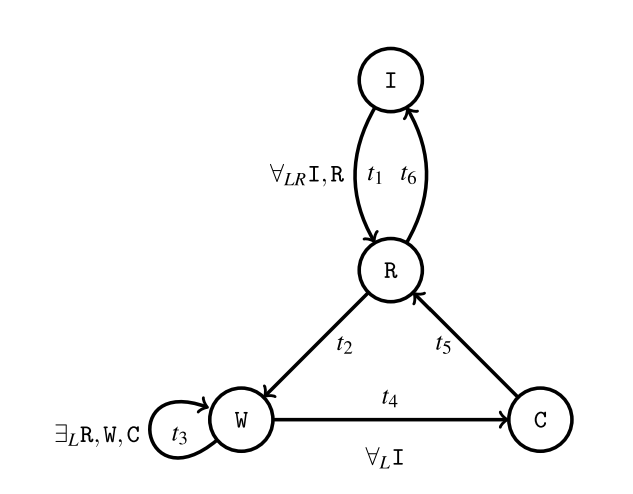
\includegraphics[width=0.3\textwidth]{./images/priority-mutex.png}
\end{center}



\begin{description}
\item[{I}] 初期状態
\item[{R}] mutex 操作をするリクエスト.
\begin{itemize}
\item 自分以外に I, R でないプロセスがいるなら I \(\longrightarrow\) R に遷移しない
\end{itemize}
\item[{W}] mutex 操作をする前にもっと優先度の高いプロセスが操作しようとしていたら待ち続ける
\item[{C}] クリティカルセクション
\end{description}
\end{frame}


\begin{frame}[label={sec:org528a844}]{例題:量化子付きの Mutex}
全てのプロセスが直線状につながっているという前提

この中の位置がプロセスの優先度に対応している
\begin{itemize}
\item 先頭に近いほど優先度が高い
\end{itemize}


例:
\begin{description}
\item[{\(\exists_{L} P\)}] 自分より左側に x があるなら,つまり自分よりも優先度の高いプロセスがいるなら,遷移する

\item[{\(\forall_{LR} P\)}] 自分より左側と右側が全て P であるなら,つまり,自分以外が全て P なら遷移する
\end{description}
\end{frame}


\section{量化子付きの遷移を含む例題の ShapeType エンコード}
\label{sec:org2bb755a}


\begin{frame}[label={sec:orge5b0515}]{量化子付きの遷移を含む例題の ShapeType エンコード}
LMNtal ShapeType は文脈自由よりも遥かに \alert{\alert{強力な文法を扱える}}
\begin{itemize}
\item (少なくとも見た目だけは) \alert{\alert{RMC の完全上位互換}} のように見える
\end{itemize}


量化子のついていない例題が
(解けるかはともかく)ShapeType へエンコードできることはほとんど明らか
\begin{itemize}
\item 量化子のついた例題に関してどうかは,あまり議論されていないように見える
\begin{itemize}
\item (直線状・リング状の例題に関しては量化子付き書き換え規則の完全上位互換である)
CSLMNtal の導入もまだ始めていない
\end{itemize}
\end{itemize}


量化子のついている例題はどうか?
\begin{itemize}
\item 多分エンコードはできる
\end{itemize}
\end{frame}



\begin{frame}[label={sec:orgb626b9e}]{存在量化子付きの遷移を含む例題の ShapeType エンコード}
存在量化子は自明
\begin{description}
\item[{RMC では}] \mbox{}\\
\alert{\alert{隣接したプロセスでない}} プロセスの存在は
存在量化子をつける必要があった
\item[{LMNtal (ShapeType) では}] \mbox{}\\
そもそも非連結グラフも扱うことができる(たぶん)
\end{description}
\end{frame}


\begin{frame}[label={sec:orgdca530c}]{全称量化子付きの遷移を含む例題の ShapeType エンコード}
全称量化子はそんなに自明でない?
\begin{itemize}
\item 「何かが無い場合に遷移する」という規則は直接は書けないが \dots{}
\end{itemize}


関数的アトムを用いて
\begin{enumerate}
\item ルールは事前に全称量化の条件をチェックしてから遷移する
\item 型の生成規則に全称量化のチェックを行うアトムも含める
\end{enumerate}
\end{frame}



\begin{frame}[label={sec:orge01eb95}]{簡略化したプロトコル}
\begin{itemize}
\item n 個のプロセスがある
\item それぞれのプロセスは
\begin{description}
\item[{i}] 初期状態
\item[{r}] リクエスト
\item[{c}] クリティカルセクション
\end{description}
の三つの状態をとる
\item i \(\longrightarrow\) r は c なプロセスがいないなら遷移可能
\item r \(\longrightarrow\) c は,\\
他にもっと優先度の高いプロセスが r, c でないなら遷移可能
\end{itemize}


同時に二つ以上 c になるものがないか?
を検証する
\end{frame}



\begin{frame}[label={sec:orgf5075e6},fragile]{全称量化付き ShapeType:システムの遷移規則}
 \footnotesize
\begin{verbatim}
% r は左側が全て i ならクリティカルセクションへ遷移可能
aquire @@
H = forallL_I([r | T]) :- H = [r | T].

% クリティカルセクションを離れる
leave @@
H = [c | T]  :- H = [i | T].

% 他に誰もクリティカルセクションに入っていないのなら,i は r になって良い
H = forallL_IL([i | forallR_IR(T)]) :- H = [r | T].
\end{verbatim}
\end{frame}




\begin{frame}[label={sec:orgfb89d01},fragile]{全称量化付き ShapeType:システムの生成規則}
 \tiny
\begin{verbatim}
defshape ps {
    ps :- head(<i*>).

    H = <i*> :- H = [i | <i*>].
    H = <i*> :- H = forallL_I(<i*>).
    H = <i*> :- H = <(i|r)*>.

    H = <(i|r)*> :- H = [i | <(i|r)*>].     % 削れるかも
    H = <(i|r)*> :- H = [r | <(i|r)*>].
    H = <(i|r)*> :- forallL_IR(<(i|r)*>).
    H = <(i|r)*> :- H = <(i|r)*c?>.

    H = <(i|r)*c?> :- H = [i | <(i|r)*c?>]. % 削れるかも
    H = <(i|r)*c?> :- H = [r | <(i|r)*c?>]. % 削れるかも
    H = <(i|r)*c?> :- H = [c | <(i|r)*c?(i|r)*>]. % cs に入るのは一つ
    H = <(i|r)*c?> :- H = <(i|r)*c?(i|r)*>.

    H = <(i|r)*c?(i|r)*> :- H = [i | <(i|r)*c?(i|r)*>].
    H = <(i|r)*c?(i|r)*> :- H = [r | <(i|r)*c?(i|r)*>].
    H = <(i|r)*c?(i|r)*> :- H = forallR_IR(<(i|r)*c?(i|r)*>]).
    H = <(i|r)*c?(i|r)*> :- H = nil.
}
\end{verbatim}
\end{frame}




\begin{frame}[label={sec:org2dd2e4c}]{全称量化付き ShapeType}
例題の感想
\begin{itemize}
\item (文法的に)あっているのかもよくわからない
\item TODO: 山本さんに相談
\end{itemize}


とはいえ,(RMC で出てくる例題レベルでは)\\
全称量化子も文法上はエンコードできる(ようだ)
\end{frame}


\section{まとめ}
\label{sec:org429b45c}

\begin{frame}[label={sec:org0861b58}]{まとめ}
RMC の手法がそのまま LMNtal に適用できるとは\textsubscript{あまり}思えないが\\
transducer という概念は重要だと思う
\begin{itemize}
\item \alert{\alert{何で抽象化するか}} ということそのものなので
\begin{itemize}
\item RMC では finite state automata = regular expression だった
\item GTS の CEGAR では(たぶん)ペトリネットだった
\item LMNtal ShapeType では LMNtal rule が \\
transducer になっているのかもしれない
(わからないが)
\end{itemize}
\end{itemize}


ShapeType は表現力的には超強力だということが理解できた
\begin{itemize}
\item 量化子も(解けるかはわからないが)扱えそう
\item ただ,どの程度効率的に解けるのかとかはわからない
\end{itemize}
\end{frame}


\begin{frame}[label={sec:org6d48b41}]{参考文献}
Handbook of Model Checking
\begin{itemize}
\item \url{https://link.springer.com/book/10.1007/978-3-319-10575-8}
\end{itemize}
\end{frame}
\end{document}
